\section{Neural Geometry Fields (NGFs)}\label{Sec:MainPart}

The Neural Geometry Fields pipeline, as proposed by Sivaram et al., consists of three main stages.  
First, a base mesh $\Sigma$ is partitioned into quadrilateral patches, forming a simplified representation of the surface.  
A learnable feature field $\Psi: \Sigma \rightarrow \mathbb{R}^F$ is then constructed, assigning a vector of $F$ real-valued components to each patch, encoding local surface properties.  
In the second stage, these features, along with the corresponding 3D positions, are passed to a neural network that predicts displacements for each surface point.  
Applying these displacements to the base mesh produces a deformed triangle mesh.  
In the final stage, the feature field and mesh parameters are optimized using an inverse rendering approach.  

In the following sections, we explore each stage in greater detail and provide illustrations to clarify the process further.

% Start of next subsection
\subsection{Surface Partitioning into Patches}

Sivaram and colleagues introduce a method for surface representation by partitioning a base mesh, denoted as $\Sigma$, into quadrilateral patches $\sigma$ (see Figure~\ref{fig:surface_processing_pipeline}).  
The process begins by simplifying the input mesh using QSlim, a robust and scalable algorithm that preserves important topological features such as holes and intersections.  
Following simplification, adjacent triangles are greedily merged into near-rectangular quadrilaterals, removing non-manifold triangles in the process.  

As a result, the method can handle non-manifold input surfaces while maintaining a consistent quadrilateral patch structure, leading to a compact and regular surface representation with fewer patches and improved organization.
% Figure 2: Surface Processing Pipeline
\usetikzlibrary{calc, shapes.geometric, arrows.meta, decorations.pathreplacing, positioning, shapes}
\begin{figure}[ht]
  \centering
  \begin{adjustbox}{center}
  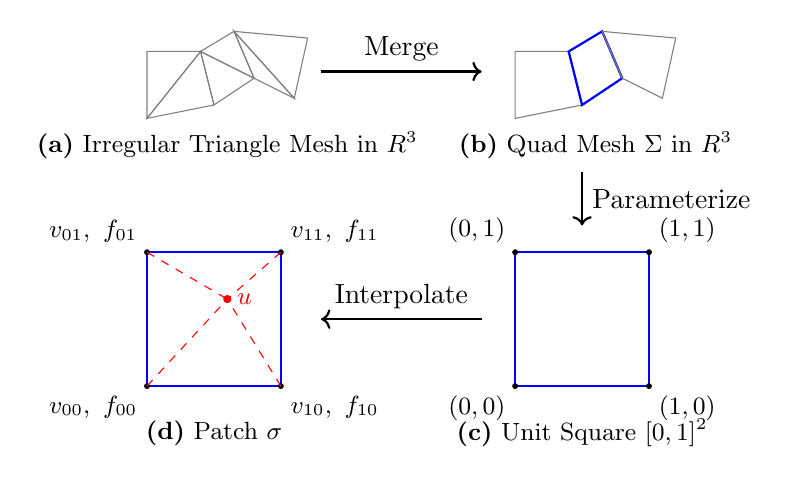
\begin{tikzpicture}[scale=0.85]

    % === Triangle Mesh (Left) ===
    \begin{scope}
      \coordinate (A) at (0,0);
      \coordinate (B) at (1,0.2);
      \coordinate (C) at (0.8,1);
      \coordinate (D) at (0,1);
      \coordinate (E) at (1.6,0.6);
      \coordinate (F) at (1.3,1.3);
      \coordinate (G) at (2.2,0.3);
      \coordinate (H) at (2.4,1.2);

      \draw[gray] (A) -- (B) -- (C) -- cycle;
      \draw[gray] (A) -- (C) -- (D) -- cycle;
      \draw[gray] (B) -- (E) -- (C) -- cycle;
      \draw[gray] (C) -- (E) -- (F) -- cycle;
      \draw[gray] (E) -- (G) -- (F) -- cycle;
      \draw[gray] (F) -- (G) -- (H) -- cycle;
      \node at (1.2, -0.4) {\small \textbf{(a)} Irregular Triangle Mesh in $\mathbb{R}^3$};
    \end{scope}

    % === Merge Arrow ===
    \draw[->, thick] (2.6,0.7) -- (5.0,0.7) node[midway, above] {Merge};

    % === Quadrilateral Mesh (Middle) ===
    \begin{scope}[xshift=5.5cm]
      \coordinate (A) at (0,0);
      \coordinate (B) at (1,0.2);
      \coordinate (C) at (0.8,1);
      \coordinate (D) at (0,1);
      \coordinate (E) at (1.6,0.6);
      \coordinate (F) at (1.3,1.3);
      \coordinate (G) at (2.2,0.3);
      \coordinate (H) at (2.4,1.2);

      \draw[gray] (A) -- (B) -- (C) -- (D) -- cycle;
      \draw[blue, thick] (B) -- (E) -- (F) -- (C) -- cycle; % highlighted patch
      \draw[gray] (E) -- (G) -- (H) -- (F) -- cycle;

      \node at (1.2, -0.4) {\small \textbf{(b)} Quad Mesh $\Sigma$ in $\mathbb{R}^3$};
    \end{scope}

    % === Down Arrow to Unit Square ===
    \draw[->, thick] (6.5,-0.8) -- (6.5,-1.6) node[midway, right] {Parameterize};

    % === Unit Square (Right) ===
    \begin{scope}[xshift=5.5cm, yshift=-4.0cm]
      \draw[blue, thick] (0,0) rectangle (2,2);
      \filldraw[black] (0,0) circle (1pt) node[anchor=north east] {\small $(0,0)$};
      \filldraw[black] (2,0) circle (1pt) node[anchor=north west] {\small $(1,0)$};
      \filldraw[black] (0,2) circle (1pt) node[anchor=south east] {\small $(0,1)$};
      \filldraw[black] (2,2) circle (1pt) node[anchor=south west] {\small $(1,1)$};
      \node at (1,-0.7) {\small \textbf{(c)} Unit Square $[0,1]^2$};
    \end{scope}

    % === Left Arrow to Feature Field ===
    \draw[->, thick] (5.0,-3) -- (2.6,-3) node[midway, above] {Interpolate};

    % === Feature Field (Left) ===
    \begin{scope}[yshift=-4.0cm]
      \draw[blue, thick] (0,0) rectangle (2,2);

      % Corner features (bold vectors), with f00 label moved outward
      \filldraw[black] (0,0) circle (1pt) node[anchor=north east] {\small $\bm{v_{00}},\ \bm{f_{00}}$};
      \filldraw[black] (2,0) circle (1pt) node[anchor=north west] {\small $\bm{v_{10}},\ \bm{f_{10}}$};
      \filldraw[black] (0,2) circle (1pt) node[anchor=south east] {\small $\bm{v_{01}},\ \bm{f_{01}}$};
      \filldraw[black] (2,2) circle (1pt) node[anchor=south west] {\small $\bm{v_{11}},\ \bm{f_{11}}$};

      % Interpolation point (u)
      \filldraw[red] (1.2,1.3) circle (1.5pt) node[right] {\small $\bm{u}$};

      % Lines from corners to interpolation point
      \foreach \x/\y in {0/0, 2/0, 0/2, 2/2} {
        \draw[dashed, red] (\x,\y) -- (1.2,1.3);
      }

      % Patch label
      \node at (1,-0.7) {\small \textbf{(d)} Patch $\sigma$};
    \end{scope}
    
  \end{tikzpicture}
  \end{adjustbox}
  \caption{Surface processing pipeline. \textbf{(a)} An irregular triangle mesh in $\mathbb{R}^3$ is simplified and merged. \textbf{(b)} The result is a quadrilateral mesh $\Sigma$. \textbf{(c)} A quadrilateral patch is parameterized over the unit square $[0,1]^2$. \textbf{(d)} This parameterization enables interpolation of geometry and features, using corner values and evaluating at an arbitrary point $\bm{u}$. Inspired by~\cite{sivaram2024}.}
  \label{fig:surface_processing_pipeline}
\end{figure}
By relying on quadrilateral patches instead of a fully triangulated mesh, the method reduces the overall patch count $|\mathcal{Q}|$ and simplifies the interpolation domain for later processing.  
This compression not only reduces storage requirements but also provides the foundation for an efficient and structured interpolation framework.  

To ensure smooth and consistent interpolation, each patch $\sigma$ must be diffeomorphic to the unit square $[0,1]^2$, meaning there exists a smooth, bijective mapping with a smooth inverse between the patch and the unit square.  
The four corner vertices of a patch are mapped as:

$(0,0) \rightarrow \mathbf{v}_{00},\ (1,0) \rightarrow \mathbf{v}_{10},\ (0,1) \rightarrow \mathbf{v}_{01},\ (1,1) \rightarrow \mathbf{v}_{11}$.  

To map an arbitrary point $\mathbf{u} = (u_x, u_y)$ within the unit square to its corresponding location on the surface patch $\sigma$, bilinear interpolation is applied:
\begin{equation}
\begin{aligned}
\sigma(\mathbf{u}) &= (1 - u_y) \left[ (1 - u_x) \cdot \mathbf{v}_{00} + u_x \cdot \mathbf{v}_{10} \right] \\
&\quad + u_y \left[ (1 - u_x) \cdot \mathbf{v}_{01} + u_x \cdot \mathbf{v}_{11} \right]
\end{aligned}
\label{func1}
\end{equation}

This yields a continuous and smooth surface.  
Conceptually, this bilinear interpolation can be thought of as first interpolating along one axis (e.g., horizontal), then the other.  
The same interpolation strategy is used to propagate feature vectors defined at each patch corner.  

Each patch corner is associated with a high-dimensional learnable feature vector.  
In the configuration used by Sivaram et al., each vector has 20 dimensions, acting as a localized descriptor of geometric or semantic properties.  
The interpolated feature value $\Psi(\mathbf{u})$ for a point $\mathbf{u}$ inside a patch is computed using bilinear blending:
\begin{equation}
\begin{aligned}
\Psi(\mathbf{u}) &= (1 - u_y) \left[ (1 - u_x) \cdot \mathbf{f}_{00} + u_x \cdot \mathbf{f}_{10} \right] \\
&\quad + u_y \left[ (1 - u_x) \cdot \mathbf{f}_{01} + u_x \cdot \mathbf{f}_{11} \right]
\end{aligned}
\label{func2}
\end{equation}

The feature field $\Psi: \Sigma \rightarrow \mathbb{R}^F$ (with $F = 20$ in the author’s setup) allows the model to smoothly interpolate semantic information across the surface.  
These features, interpolated at points on the patch, can be sampled across the surface for later neural processing stages.  

The following section describes how this patch-based representation is used to generate detailed geometry through a neural deformation model, including the role of tessellation, feature encoding and the architecture of the Multi-Layer Perceptron.  

% Start of next section
\subsection{Patch-Based Sampling and Feature Encoding}

Building on the quadrilateral patch structure introduced before, Sivaram et al.\ develop a neural representation that enables fine-grained geometry reconstruction over the base mesh.  
Each patch, defined as a bilinear map from the unit square $[0,1]^2$ to a region on the simplified surface, provides a consistent local domain for both geometric interpolation and neural processing.  

To capture detailed shape variations across the surface, the method samples a dense grid of points within each patch.  
A regular $k \times k$ grid is overlaid on the unit square domain, producing a set of parametric coordinates $\mathbf{u}_{ij} \in [0,1]^2$ for $i,j \in \{0, \ldots, k - 1\}$.  
The value of $k$ determines the spatial sampling resolution within each patch and is configurable depending on the desired level of detail.  
The paper evaluates several settings, such as $k \in \{4, 8, 12, 16\}$.  
These samples form the foundation for evaluating both geometry and features across the patch.

% Start of subsection
\subsubsection{Jittered Sampling for Detail and Regularization}

While regular sampling places points at fixed, evenly spaced positions $\hat{\mathbf{u}} = \langle i, j \rangle / (k - 1)$, this uniform layout can lead to aliasing and oversmoothing, particularly in areas with high-frequency geometric detail.  
To address this, jittered sampling is applied by perturbing interior sample points with small, random offsets drawn from a disk-shaped distribution:  
\[
\mathbf{u} \sim \hat{\mathbf{u}} + D(\omega)
\]  
where $D(\omega)$ samples uniformly from a disk of radius $\omega$.  
This introduces local variation without disrupting the patchs overall structure.  

To ensure mesh consistency and continuity, two constraints are enforced:  
\begin{itemize}
  \item \textbf{Boundary Alignment:} To preserve continuity across adjacent patches, boundary points are kept fixed ($\omega = 0$), ensuring precise alignment.  
  \item \textbf{Jitter Constraint:} The jitter radius is limited to $\omega < 0.5k^{-1}$, effectively avoiding triangle fold-overs and mesh inversions.  
\end{itemize}

This stochastic sampling approach improves generalization by reducing overfitting to a fixed grid layout.  
It promotes smoother deformations and higher robustness, especially in low-resolution areas where uniform sampling may miss details.  
This process is illustrated in Figure~\ref{fig:jittered-sampling}, showing how jittered sampling enhances geometric flexibility while maintaining continuity constraints.

\usetikzlibrary{arrows.meta, shapes.geometric}
\begin{figure}[h!]
  \centering
  \begin{adjustbox}{center}
  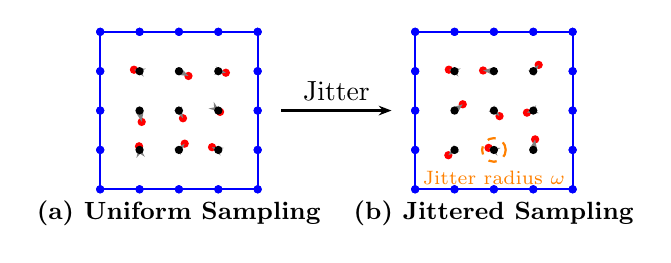
\begin{tikzpicture}[scale=1, >={Stealth[scale=0.7]}, line width=0.6pt]

  % Parameters
  \def\gridSize{4} % number of intervals per side
  \def\patchSize{2} % side length of patch
  \def\jitterRadius{0.15} % max jitter radius

  % Helper: Draw uniform grid points
  \newcommand{\drawGridPoints}[2]{ % #1 = xshift, #2 = jitter flag (true/false)
    \foreach \i in {0,...,\gridSize} {
      \foreach \j in {0,...,\gridSize} {
        \pgfmathsetmacro{\x}{(\i/\gridSize)*\patchSize}
        \pgfmathsetmacro{\y}{(\j/\gridSize)*\patchSize}
        % Boundary detection
        \ifnum\i=0
          \def\isBoundary{1}
        \else
          \ifnum\i=\gridSize
            \def\isBoundary{1}
          \else
            \ifnum\j=0
              \def\isBoundary{1}
            \else
              \ifnum\j=\gridSize
                \def\isBoundary{1}
              \else
                \def\isBoundary{0}
              \fi
            \fi
          \fi
        \fi

        % Draw points:
        \ifthenelse{\equal{#2}{true}}{
          % Jitter points on right panel only if not boundary
          \ifnum\isBoundary=0
            % jitter by random angle and radius inside disk
            \pgfmathparse{360*random()} \let\angle\pgfmathresult
            \pgfmathparse{\jitterRadius*sqrt(random())} \let\radius\pgfmathresult
            \pgfmathsetmacro{\jx}{\radius*cos(\angle)}
            \pgfmathsetmacro{\jy}{\radius*sin(\angle)}

            % Draw original point in gray
            \fill[gray] (#1+\x, \y) circle (0.8pt);
            % Draw jittered point in red
            \fill[red] (#1+\x+\jx, \y+\jy) circle (1.5pt);
            % Draw arrow from original to jittered
            \draw[->, gray] (#1+\x, \y) -- (#1+\x+\jx, \y+\jy);
          \else
            % Boundary points: no jitter, blue dots
            \fill[blue] (#1+\x, \y) circle (1.5pt);
          \fi
        }{
          % Left panel: uniform grid points black or blue for boundary
          \ifnum\isBoundary=1
            \fill[blue] (#1+\x, \y) circle (1.5pt);
          \else
            \fill[black] (#1+\x, \y) circle (1.5pt);
          \fi
        }
      }
    }
  }

  % Left panel: Uniform sampling
  \begin{scope}[xshift=0cm]
    \draw[blue, thick] (0,0) rectangle (\patchSize,\patchSize);
    \drawGridPoints{0}{false}
    \node at (\patchSize/2,-0.3) {\small \textbf{(a) Uniform Sampling}};
  \end{scope}

  % Arrow to right panel
  \draw[->, thick] (\patchSize+0.3,\patchSize/2) -- (\patchSize+1.7,\patchSize/2) node[midway, above] {Jitter};

  % Right panel: Jittered sampling
  \begin{scope}[xshift=4cm]
    \draw[blue, thick] (0,0) rectangle (\patchSize,\patchSize);
    \drawGridPoints{0}{true}
    \node at (\patchSize/2,-0.3) {\small \textbf{(b) Jittered Sampling}};

    % Draw jitter radius disk around one interior point (e.g., grid point (2,1))
    \pgfmathsetmacro{\cx}{(2/\gridSize)*\patchSize}
    \pgfmathsetmacro{\cy}{(1/\gridSize)*\patchSize}
    \draw[thick, dashed, orange] (\cx,\cy) circle (\jitterRadius);
    \node[orange] at (\cx, \cy + \jitterRadius - 0.5) {\scriptsize Jitter radius \(\omega\)};
  \end{scope}

  \end{tikzpicture}
  \end{adjustbox}
  \caption{Illustration of jittered sampling. (a) Uniform grid samples on a patch with boundary points in blue and interior grid points in black. (b) Points after applying jitter within a disk of radius \(\omega\) (orange dashed circle) around interior points. Boundary points remain blue and are not jittered. Original points before jittering are shown as small gray dots and jittered points are shown in red with arrows indicating displacement vectors.}
  \label{fig:jittered-sampling}
\end{figure}

% Start of next subsection
\subsubsection{Feature Evaluation and Positional Encoding}

After the application of jittered sampling, at each of these samples, two key quantities are computed:  
\begin{itemize}
  \item The 3D position $\sigma(\mathbf{u}_{ij})$,  
  \item The interpolated feature vector $\Psi(\mathbf{u}_{ij})$.  
\end{itemize}

To enable the network to learn surface deformations, the sampled geometry and feature values are transformed through a high-frequency positional encoding~\cite{mildenhall2020}.  
Specifically, each input point is encoded as:  
\begin{equation}
\begin{aligned}
\text{enc}(\sigma(\mathbf{u}), \Psi(\mathbf{u})) = \big(&
\sin(2^0 \sigma(\mathbf{u})), \cos(2^0 \sigma(\mathbf{u})), \ldots, \\
&\sin(2^L \sigma(\mathbf{u})), \cos(2^L \sigma(\mathbf{u})), 
\Psi(\mathbf{u})
\big)
\end{aligned}
\label{func3}
\end{equation}

where \( L \) denotes the number of frequency bands.  
In the configuration used by Sivaram and colleagues, \( L = 8 \).

This encoding combines geometric location with semantic features in a form suitable for learning complex local surface variations.  
With a structured input representation defined, the next step is to use this data to predict detailed 3D geometry through learned surface deformation.  

% Start of next subsection
\subsubsection{Neural Surface Deformation with MLP}

To reconstruct high-fidelity surface geometry, the model employs a neural deformation module based on a Multi-Layer Perceptron.  
The MLP receives as input the geometric coordinates of a surface sample along with learned feature embeddings and predicts fine-grained displacements to locally refine a coarse base mesh.

Formally, the deformed 3D position $\Lambda(\mathbf{u})$ of a point $\mathbf{u}$ is given by:
\begin{equation*}
\Lambda(\mathbf{u}) = \sigma(\mathbf{u}) + \text{MLP}_\theta\left( \text{enc}(\sigma(\mathbf{u}), \Psi(\mathbf{u})) \right)
\end{equation*}

where $\sigma(\mathbf{u})$ (equation~\ref{func1}) is the jittered 3D coordinate of the point on the base surface, $\Psi(\mathbf{u})$ (equation~\ref{func2}) denotes its corresponding feature vector and $\text{enc}(\cdot)$ (equation~\ref{func3}) is the encoder that fuses geometric and feature information.
The MLP learns to predict displacements that adjust $\sigma(\mathbf{u})$ to better match the target high-resolution geometry.
The complete process is illustrated in Figure~\ref{fig:neural_displacement}, which shows how a sampled point $\mathbf{u}_i$ is transformed into a deformed position $\mathbf{x}_i$ through encoding and MLP-based displacement.

\begin{figure}[ht]
  \centering
  \begin{adjustbox}{center}
  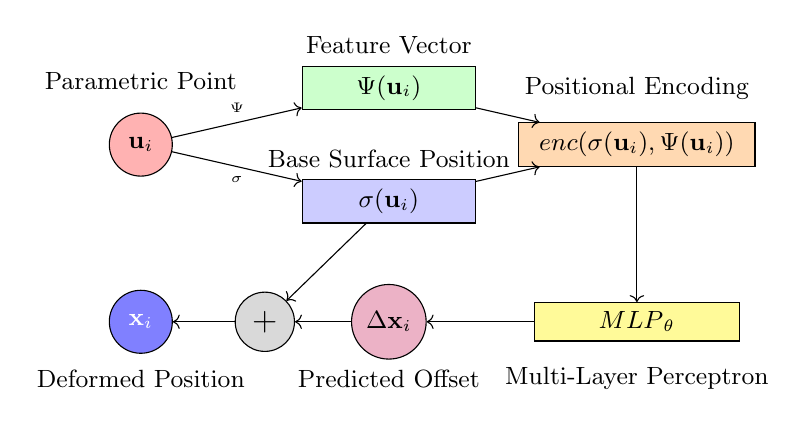
\begin{tikzpicture}[scale=0.9]

    % Sample point u_i
    \node[draw, circle, fill=red!30, minimum size=0.8cm] (u) at (0,0) {\small $\mathbf{u}_i$};
    \node at (0,0.9) {\small Parametric Point};

    % Psi(u)
    \node[draw, rectangle, fill=green!20, minimum width=2.2cm] (psi) at (3.5,0.8) {\small $\Psi(\mathbf{u}_i)$};
    \node at (3.5,1.4) {\small Feature Vector};

    % Sigma(u)
    \node[draw, rectangle, fill=blue!20, minimum width=2.2cm] (sigma) at (3.5,-0.8) {\small $\sigma(\mathbf{u}_i)$};
    \node at (3.5,-0.2) {\small Base Surface Position};

    % Encoding node
    \node[draw, rectangle, fill=orange!30, minimum width=3cm] (enc) at (7,0) {\small $\text{enc}(\sigma(\mathbf{u}_i), \Psi(\mathbf{u}_i))$};
    \node at (7,0.8) {\small Positional Encoding};

    % MLP node
    \node[draw, rectangle, fill=yellow!40, minimum width=2.6cm] (mlp) at (7,-2.5) {\small $\text{MLP}_\theta$};
    \node at (7,-3.3) {\small Multi-Layer Perceptron};

    % Displacement vector
    \node[draw, circle, fill=purple!30, minimum size=0.8cm] (dx) at (3.5,-2.5) {\small $\Delta \mathbf{x}_i$};
    \node at (3.5,-3.3) {\small Predicted Offset};

    % Plus node for summing sigma(ui) and delta_x (smaller + symbol)
    \node[draw, circle, fill=gray!30, minimum size=0.6cm] (plus) at (1.75,-2.5) {\large $+$};

    % Final position
    \node[draw, circle, fill=blue!50, text=white, minimum size=0.8cm] (x) at (0,-2.5) {\small $\mathbf{x}_i$};
    \node at (0,-3.3) {\small Deformed Position};

    % Arrows
    \draw[->] (u) -- (psi) node[midway, above] {\tiny $\Psi$};
    \draw[->] (u) -- (sigma) node[midway, below] {\tiny $\sigma$};
    \draw[->] (sigma) -- (enc);
    \draw[->] (psi) -- (enc);
    \draw[->] (enc) -- (mlp);
    \draw[->] (mlp) -- (dx);
    \draw[->] (sigma) -- (plus);
    \draw[->] (dx) -- (plus);
    \draw[->] (plus) -- (x);

  \end{tikzpicture}
  \end{adjustbox}
  \caption{Neural displacement pipeline for a sampled point $\mathbf{u}_i$. The point is mapped to a corresponding feature vector $\Psi(\mathbf{u}_i)$ and a base surface position $\sigma(\mathbf{u}_i)$. These inputs are passed through a positional encoding and a learned MLP to produce a displacement vector $\Delta \mathbf{x}_i$. The final deformed position $\mathbf{x}_i$ is obtained by adding the base position and the predicted offset, shown by the plus symbol.}
  \label{fig:neural_displacement}
\end{figure}

The MLP is implemented as a feedforward neural network with two hidden layers, each containing 64 units.  
Although the activation function is not explicitly specified by the original authors, standard choices such as ReLU~\cite{nair2010} or GELU~\cite{hendrycks2023} are likely used to enable the modeling of complex nonlinear deformations.  
These nonlinearities are essential for capturing complex surface details beyond what can be represented by linear displacements.

Both the MLP parameters $\theta$ and the per-vertex feature embeddings are optimized jointly during training.  
The training process is supervised using differentiable rendering, which allows image-space losses to be backpropagated through the rendering pipeline and used to update the 3D geometry.  
The method leverages \textsc{NVDIFFRAST}~\cite{laine2020}, a GPU-accelerated differentiable rasterizer that supports rendering triangle meshes while computing gradients with respect to vertex positions and attributes.

To provide rich and diverse supervision, each 3D object is rendered from 200 virtual viewpoints, evenly sampled on a sphere surrounding the object.  
Rendering is performed using multi-layer depth buffers, where each pixel can record information for up to three surfaces along a viewing ray.  
This strategy enables accurate modeling of occlusions and semi-transparent regions.  
To maintain computational efficiency and manage GPU memory, viewpoints are processed in batches of 10.

Optimization is performed using the Adam optimizer~\cite{kingma2017}, with a fixed learning rate of $10^{-3}$.  
Adam's adaptive learning rates and moment estimation improve convergence speed and stability over standard gradient descent.

This MLP-based deformation framework, trained with differentiable rendering and dense multi-view supervision, enables the model to reconstruct fine surface details with strong view consistency and geometric plausibility.

% Start of next subsection
\subsection{Loss Functions for Deformation Training}

With the deformation network defined, training proceeds by minimizing a combination of geometric and image-based loss functions designed to enforce both reconstruction fidelity and regularization, as proposed by Sivaram et al.

Unlike traditional pipelines that rely solely on image supervision, this method also utilizes ground truth geometric information, specifically surface normals, as a guiding signal.
Vertex normals are computed on the predicted mesh using cross products of adjacent triangle edges.
During differentiable rasterization, these per-vertex normals are interpolated across pixels to produce normal buffers for both the predicted surface $\Sigma$ and the reference surface $\Gamma$.

The image-space normal consistency loss is then defined as:
\[
L_{\text{normal}} = \frac{1}{|\mathcal{N}(*)|} \left\| \mathcal{N}(\Gamma) - \mathcal{N}(\Sigma) \right\|_1
\]

To promote smooth, uniform geometry and prevent artifacts like vertex clustering, a Laplacian regularization term is added:
\[
L_{\text{laplacian}} = \frac{1}{|V|} \left\| \mathcal{L}_V \right\|_1
\]

where $\mathcal{L}$ is the uniform mesh Laplacian operator applied to the set of sampled vertices $V$.

The total loss function is:
\[
L_{\text{total}} = L_{\text{normal}} + L_{\text{laplacian}}
\]

This formulation encourages the reconstructed mesh to be both visually accurate and structurally regular.

% Start of next subsection
\subsubsection{Mesh Construction and Optimization}

Once the deformed 3D points are predicted by the MLP, they are converted into a coherent surface mesh.
This is done by triangulating the regular $k \times k$ sampling grid defined within each surface patch.
Each square cell in the grid is consistently split along a diagonal (e.g., from bottom-left to top-right), ensuring uniform triangulation across all patches.

To guarantee global mesh consistency, adjacent patches share boundary vertices and maintain aligned sampling grids.
This alignment ensures that there are no gaps, cracks or overlaps at the seams between patches, resulting in a watertight mesh topology \cite{sivaram2024}.
Watertightness means the mesh forms a continuous, closed surface without holes or gaps. It is essential for downstream tasks such as differentiable rendering, physical simulation and mesh-based editing, where topological correctness directly affects visual and functional quality.

This structured triangulation strategy provides an efficient and robust mechanism for converting locally deformed surface samples into a globally consistent 3D mesh representation.

% Start of next subsection
\subsubsection{Inverse Rendering}

To improve reconstructed geometry beyond coarse alignment, NGFs incorporates inverse rendering based on differentiable rasterization.
Instead of relying solely on geometric losses, such as Chamfer distance or signed distance fields, which are sensitive to noise and sampling density, the method uses appearance-based supervision from multi-view imagery~\cite{Hasselgren2021}.

A differentiable rasterizer renders images of the predicted mesh and compares them to ground-truth views.
The resulting appearance loss propagates gradients through the rendering pipeline, enabling joint optimization of both geometry and appearance.
This strategy enhances fidelity in complex or partially occluded regions where geometric losses often fail.

Training follows a coarse-to-fine optimization schedule.
Starting from a low tessellation level $k$, the model gradually increases sampling density, first capturing global structure, then refining local details.
At each level, the mesh $M$ has fixed connectivity defined by a regular triangulation of the sampled patch grid~\cite{sivaram2024}.

The vertex positions of $M$ are differentiable with respect to:
\begin{itemize}
    \item The patch corner positions $V$,
    \item The per-vertex feature vectors $F$,
    \item The deformation network parameters $\theta$.
\end{itemize}

This full differentiability ensures effective gradient flow throughout the optimization, enabling the network to jointly refine shape and appearance.
By integrating differentiable rasterization with multi-view consistency, the model achieves reconstructions that are both geometrically accurate and visually coherent across all observed viewpoints.

In practice, the runtime performance of the inverse rendering pipeline is efficient. 
At a resolution of $k = 16$, training with 2,500 patches requires approximately 12 minutes and surface extraction takes around 21.22 milliseconds, measured on an RTX 2080 Ti GPU.

These results highlight the controllability of the NGF training and inference, even with the added complexity of differentiable rendering, on standard consumer-grade hardware.